% This file is generated by the MATLAB m-file laprint.m. It can be included
% into LaTeX documents using the packages graphicx, color and psfrag.
% It is accompanied by a postscript file. A sample LaTeX file is:
%    \documentclass{article}\usepackage{graphicx,color,psfrag}
%    \begin{document}% This file is generated by the MATLAB m-file laprint.m. It can be included
% into LaTeX documents using the packages graphicx, color and psfrag.
% It is accompanied by a postscript file. A sample LaTeX file is:
%    \documentclass{article}\usepackage{graphicx,color,psfrag}
%    \begin{document}% This file is generated by the MATLAB m-file laprint.m. It can be included
% into LaTeX documents using the packages graphicx, color and psfrag.
% It is accompanied by a postscript file. A sample LaTeX file is:
%    \documentclass{article}\usepackage{graphicx,color,psfrag}
%    \begin{document}% This file is generated by the MATLAB m-file laprint.m. It can be included
% into LaTeX documents using the packages graphicx, color and psfrag.
% It is accompanied by a postscript file. A sample LaTeX file is:
%    \documentclass{article}\usepackage{graphicx,color,psfrag}
%    \begin{document}\input{L2comp}\end{document}
% See http://www.mathworks.de/matlabcentral/fileexchange/loadFile.do?objectId=4638
% for recent versions of laprint.m.
%
% created by:           LaPrint version 3.16 (13.9.2004)
% created on:           29-May-2012 12:33:24
% eps bounding box:     15 cm x 11.1094 cm
% comment:              
%
\begin{psfrags}%
\psfragscanon%
%
% text strings:
\psfrag{s05}[t][t]{\color[rgb]{0,0,0}\setlength{\tabcolsep}{0pt}\begin{tabular}{c}$M$\end{tabular}}%
\psfrag{s06}[b][b][1][180]{\color[rgb]{0,0,0}\setlength{\tabcolsep}{0pt}\begin{tabular}{c}$\epsilon_{2}$
error\end{tabular}}%
\psfrag{s10}[][]{\color[rgb]{0,0,0}\setlength{\tabcolsep}{0pt}\begin{tabular}{c}
\end{tabular}}%
\psfrag{s11}[][]{\color[rgb]{0,0,0}\setlength{\tabcolsep}{0pt}\begin{tabular}{c}
\end{tabular}}%
%
\psfrag{s13}[l][l]{\color[rgb]{0,0,0}$\tpbs^0_p$}%
\psfrag{s14}[l][l]{\color[rgb]{0,0,0}$\tpbs^1_p$-\small{interp.}}%
\psfrag{s15}[l][l]{\color[rgb]{0,0,0}$\tpbs^3_p$-\small{interp.}}%
\psfrag{s16}[l][l]{\color[rgb]{0,0,0}$\tpbs^3_p$-\small{quasi.}}%
%
\psfrag{s17}[l][l]{\color[rgb]{0,0,0}$V_{\lattice{H},p}^0$}%
\psfrag{s18}[l][l]{\color[rgb]{0,0,0}$\bccbs{2}_p$-\small{interp.}}%
\psfrag{s19}[l][l]{\color[rgb]{0,0,0}$\bccbs{4}_p$-\small{interp.}}%
\psfrag{s20}[l][l]{\color[rgb]{0,0,0}$\bccbs{4}_p$-\small{quasi.}}%
%
% slopes
% CC slopes
\psfrag{m5}[r][r]{\color[rgb]{0,0,0}$0.9963$}%
\psfrag{m6}[r][r]{\color[rgb]{0,0,0}$1.9930$}%
\psfrag{m7}[r][r]{\color[rgb]{0,0,0}$3.9468$}%
\psfrag{m8}[r][r]{\color[rgb]{0,0,0}$4.0596$}%
%
%BCC slopes
\psfrag{m1}[r][r]{\color[rgb]{0,0,0}$1.0021$}%
\psfrag{m2}[r][r]{\color[rgb]{0,0,0}$2.0011$}%
\psfrag{m3}[r][r]{\color[rgb]{0,0,0}$3.9796$}%
\psfrag{m4}[r][r]{\color[rgb]{0,0,0}$4.0470$}%
%
%
\psfrag{H1}[l][l]{\color[rgb]{0,0,0}\textbf{BCC}}%
\psfrag{H2}[l][l]{\color[rgb]{0,0,0}\textbf{CC}}%
% xticklabels:
\psfrag{x11}[t][t]{1}%
\psfrag{x01}[t][t]{${16}$}%
\psfrag{x02}[t][t]{${32}$}%
\psfrag{x03}[t][t]{${64}$}%
\psfrag{x04}[t][t]{${128}$}%
\psfrag{x05}[t][t]{${256}$}%
\psfrag{x06}[t][t]{${512}$}%
%
% yticklabels:
\psfrag{v08}[r][r]{$10^{1}$}%
\psfrag{v07}[r][r]{$10^{0}$}%
\psfrag{v06}[r][r]{$10^{-1}$}%
\psfrag{v05}[r][r]{$10^{-2}$}%
\psfrag{v04}[r][r]{$10^{-3}$}%
\psfrag{v03}[r][r]{$10^{-4}$}%
\psfrag{v02}[r][r]{$10^{-5}$}%
\psfrag{v01}[r][r]{$10^{-6}$}%
%
% Figure:
\resizebox{6cm}{!}{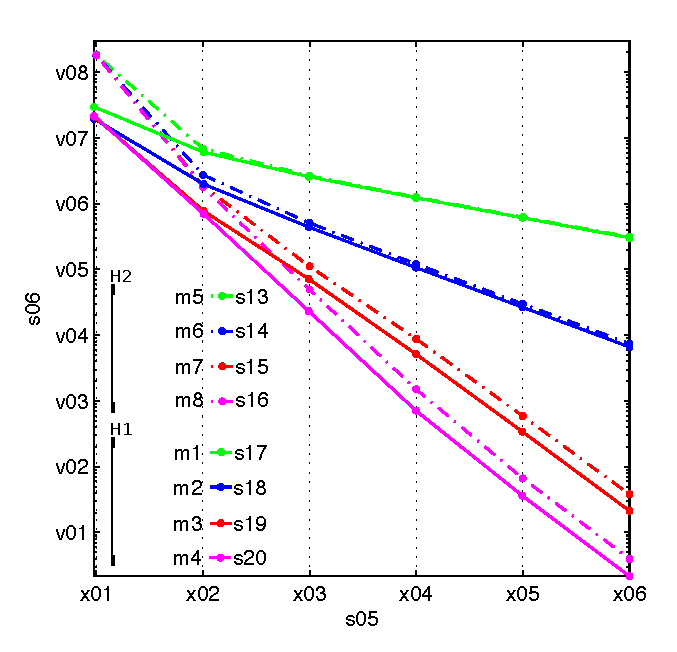
\includegraphics{L2comp.eps}}%
\end{psfrags}%
%
% End L2comp.tex
\end{document}
% See http://www.mathworks.de/matlabcentral/fileexchange/loadFile.do?objectId=4638
% for recent versions of laprint.m.
%
% created by:           LaPrint version 3.16 (13.9.2004)
% created on:           29-May-2012 12:33:24
% eps bounding box:     15 cm x 11.1094 cm
% comment:              
%
\begin{psfrags}%
\psfragscanon%
%
% text strings:
\psfrag{s05}[t][t]{\color[rgb]{0,0,0}\setlength{\tabcolsep}{0pt}\begin{tabular}{c}$M$\end{tabular}}%
\psfrag{s06}[b][b][1][180]{\color[rgb]{0,0,0}\setlength{\tabcolsep}{0pt}\begin{tabular}{c}$\epsilon_{2}$
error\end{tabular}}%
\psfrag{s10}[][]{\color[rgb]{0,0,0}\setlength{\tabcolsep}{0pt}\begin{tabular}{c}
\end{tabular}}%
\psfrag{s11}[][]{\color[rgb]{0,0,0}\setlength{\tabcolsep}{0pt}\begin{tabular}{c}
\end{tabular}}%
%
\psfrag{s13}[l][l]{\color[rgb]{0,0,0}$\tpbs^0_p$}%
\psfrag{s14}[l][l]{\color[rgb]{0,0,0}$\tpbs^1_p$-\small{interp.}}%
\psfrag{s15}[l][l]{\color[rgb]{0,0,0}$\tpbs^3_p$-\small{interp.}}%
\psfrag{s16}[l][l]{\color[rgb]{0,0,0}$\tpbs^3_p$-\small{quasi.}}%
%
\psfrag{s17}[l][l]{\color[rgb]{0,0,0}$V_{\lattice{H},p}^0$}%
\psfrag{s18}[l][l]{\color[rgb]{0,0,0}$\bccbs{2}_p$-\small{interp.}}%
\psfrag{s19}[l][l]{\color[rgb]{0,0,0}$\bccbs{4}_p$-\small{interp.}}%
\psfrag{s20}[l][l]{\color[rgb]{0,0,0}$\bccbs{4}_p$-\small{quasi.}}%
%
% slopes
% CC slopes
\psfrag{m5}[r][r]{\color[rgb]{0,0,0}$0.9963$}%
\psfrag{m6}[r][r]{\color[rgb]{0,0,0}$1.9930$}%
\psfrag{m7}[r][r]{\color[rgb]{0,0,0}$3.9468$}%
\psfrag{m8}[r][r]{\color[rgb]{0,0,0}$4.0596$}%
%
%BCC slopes
\psfrag{m1}[r][r]{\color[rgb]{0,0,0}$1.0021$}%
\psfrag{m2}[r][r]{\color[rgb]{0,0,0}$2.0011$}%
\psfrag{m3}[r][r]{\color[rgb]{0,0,0}$3.9796$}%
\psfrag{m4}[r][r]{\color[rgb]{0,0,0}$4.0470$}%
%
%
\psfrag{H1}[l][l]{\color[rgb]{0,0,0}\textbf{BCC}}%
\psfrag{H2}[l][l]{\color[rgb]{0,0,0}\textbf{CC}}%
% xticklabels:
\psfrag{x11}[t][t]{1}%
\psfrag{x01}[t][t]{${16}$}%
\psfrag{x02}[t][t]{${32}$}%
\psfrag{x03}[t][t]{${64}$}%
\psfrag{x04}[t][t]{${128}$}%
\psfrag{x05}[t][t]{${256}$}%
\psfrag{x06}[t][t]{${512}$}%
%
% yticklabels:
\psfrag{v08}[r][r]{$10^{1}$}%
\psfrag{v07}[r][r]{$10^{0}$}%
\psfrag{v06}[r][r]{$10^{-1}$}%
\psfrag{v05}[r][r]{$10^{-2}$}%
\psfrag{v04}[r][r]{$10^{-3}$}%
\psfrag{v03}[r][r]{$10^{-4}$}%
\psfrag{v02}[r][r]{$10^{-5}$}%
\psfrag{v01}[r][r]{$10^{-6}$}%
%
% Figure:
\resizebox{6cm}{!}{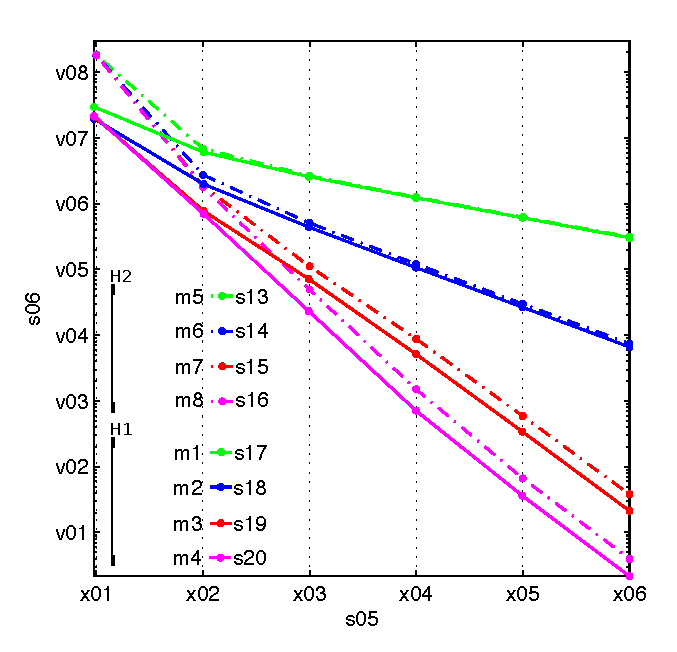
\includegraphics{L2comp.eps}}%
\end{psfrags}%
%
% End L2comp.tex
\end{document}
% See http://www.mathworks.de/matlabcentral/fileexchange/loadFile.do?objectId=4638
% for recent versions of laprint.m.
%
% created by:           LaPrint version 3.16 (13.9.2004)
% created on:           29-May-2012 12:33:24
% eps bounding box:     15 cm x 11.1094 cm
% comment:              
%
\begin{psfrags}%
\psfragscanon%
%
% text strings:
\psfrag{s05}[t][t]{\color[rgb]{0,0,0}\setlength{\tabcolsep}{0pt}\begin{tabular}{c}$M$\end{tabular}}%
\psfrag{s06}[b][b][1][180]{\color[rgb]{0,0,0}\setlength{\tabcolsep}{0pt}\begin{tabular}{c}$\epsilon_{2}$
error\end{tabular}}%
\psfrag{s10}[][]{\color[rgb]{0,0,0}\setlength{\tabcolsep}{0pt}\begin{tabular}{c}
\end{tabular}}%
\psfrag{s11}[][]{\color[rgb]{0,0,0}\setlength{\tabcolsep}{0pt}\begin{tabular}{c}
\end{tabular}}%
%
\psfrag{s13}[l][l]{\color[rgb]{0,0,0}$\tpbs^0_p$}%
\psfrag{s14}[l][l]{\color[rgb]{0,0,0}$\tpbs^1_p$-\small{interp.}}%
\psfrag{s15}[l][l]{\color[rgb]{0,0,0}$\tpbs^3_p$-\small{interp.}}%
\psfrag{s16}[l][l]{\color[rgb]{0,0,0}$\tpbs^3_p$-\small{quasi.}}%
%
\psfrag{s17}[l][l]{\color[rgb]{0,0,0}$V_{\lattice{H},p}^0$}%
\psfrag{s18}[l][l]{\color[rgb]{0,0,0}$\bccbs{2}_p$-\small{interp.}}%
\psfrag{s19}[l][l]{\color[rgb]{0,0,0}$\bccbs{4}_p$-\small{interp.}}%
\psfrag{s20}[l][l]{\color[rgb]{0,0,0}$\bccbs{4}_p$-\small{quasi.}}%
%
% slopes
% CC slopes
\psfrag{m5}[r][r]{\color[rgb]{0,0,0}$0.9963$}%
\psfrag{m6}[r][r]{\color[rgb]{0,0,0}$1.9930$}%
\psfrag{m7}[r][r]{\color[rgb]{0,0,0}$3.9468$}%
\psfrag{m8}[r][r]{\color[rgb]{0,0,0}$4.0596$}%
%
%BCC slopes
\psfrag{m1}[r][r]{\color[rgb]{0,0,0}$1.0021$}%
\psfrag{m2}[r][r]{\color[rgb]{0,0,0}$2.0011$}%
\psfrag{m3}[r][r]{\color[rgb]{0,0,0}$3.9796$}%
\psfrag{m4}[r][r]{\color[rgb]{0,0,0}$4.0470$}%
%
%
\psfrag{H1}[l][l]{\color[rgb]{0,0,0}\textbf{BCC}}%
\psfrag{H2}[l][l]{\color[rgb]{0,0,0}\textbf{CC}}%
% xticklabels:
\psfrag{x11}[t][t]{1}%
\psfrag{x01}[t][t]{${16}$}%
\psfrag{x02}[t][t]{${32}$}%
\psfrag{x03}[t][t]{${64}$}%
\psfrag{x04}[t][t]{${128}$}%
\psfrag{x05}[t][t]{${256}$}%
\psfrag{x06}[t][t]{${512}$}%
%
% yticklabels:
\psfrag{v08}[r][r]{$10^{1}$}%
\psfrag{v07}[r][r]{$10^{0}$}%
\psfrag{v06}[r][r]{$10^{-1}$}%
\psfrag{v05}[r][r]{$10^{-2}$}%
\psfrag{v04}[r][r]{$10^{-3}$}%
\psfrag{v03}[r][r]{$10^{-4}$}%
\psfrag{v02}[r][r]{$10^{-5}$}%
\psfrag{v01}[r][r]{$10^{-6}$}%
%
% Figure:
\resizebox{6cm}{!}{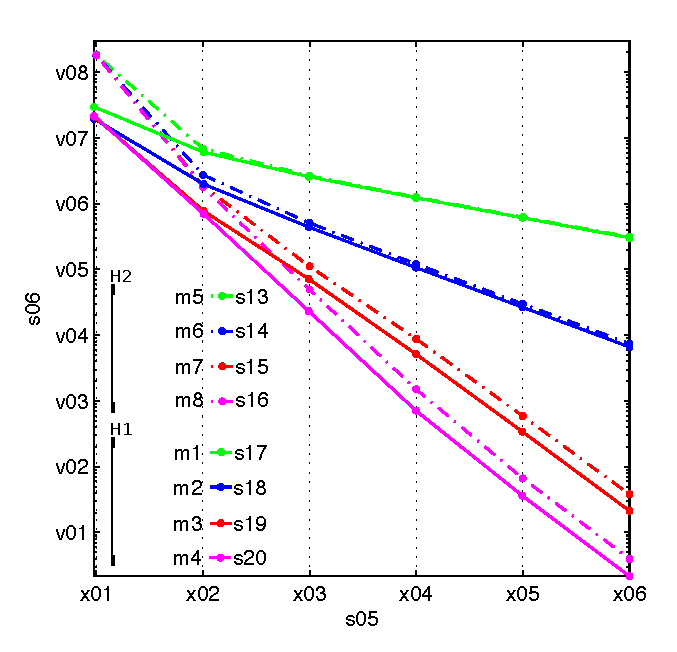
\includegraphics{L2comp.eps}}%
\end{psfrags}%
%
% End L2comp.tex
\end{document}
% See http://www.mathworks.de/matlabcentral/fileexchange/loadFile.do?objectId=4638
% for recent versions of laprint.m.
%
% created by:           LaPrint version 3.16 (13.9.2004)
% created on:           29-May-2012 12:33:24
% eps bounding box:     15 cm x 11.1094 cm
% comment:              
%
\begin{psfrags}%
\psfragscanon%
%
% text strings:
\psfrag{s05}[t][t]{\color[rgb]{0,0,0}\setlength{\tabcolsep}{0pt}\begin{tabular}{c}$M$\end{tabular}}%
\psfrag{s06}[b][b][1][180]{\color[rgb]{0,0,0}\setlength{\tabcolsep}{0pt}\begin{tabular}{c}$\epsilon_{2}$
error\end{tabular}}%
\psfrag{s10}[][]{\color[rgb]{0,0,0}\setlength{\tabcolsep}{0pt}\begin{tabular}{c}
\end{tabular}}%
\psfrag{s11}[][]{\color[rgb]{0,0,0}\setlength{\tabcolsep}{0pt}\begin{tabular}{c}
\end{tabular}}%
%
\psfrag{s13}[l][l]{\color[rgb]{0,0,0}$\tpbs^0_p$}%
\psfrag{s14}[l][l]{\color[rgb]{0,0,0}$\tpbs^1_p$-\small{interp.}}%
\psfrag{s15}[l][l]{\color[rgb]{0,0,0}$\tpbs^3_p$-\small{interp.}}%
\psfrag{s16}[l][l]{\color[rgb]{0,0,0}$\tpbs^3_p$-\small{quasi.}}%
%
\psfrag{s17}[l][l]{\color[rgb]{0,0,0}$V_{\lattice{H},p}^0$}%
\psfrag{s18}[l][l]{\color[rgb]{0,0,0}$\bccbs{2}_p$-\small{interp.}}%
\psfrag{s19}[l][l]{\color[rgb]{0,0,0}$\bccbs{4}_p$-\small{interp.}}%
\psfrag{s20}[l][l]{\color[rgb]{0,0,0}$\bccbs{4}_p$-\small{quasi.}}%
%
% slopes
% CC slopes
\psfrag{m5}[r][r]{\color[rgb]{0,0,0}$0.9963$}%
\psfrag{m6}[r][r]{\color[rgb]{0,0,0}$1.9930$}%
\psfrag{m7}[r][r]{\color[rgb]{0,0,0}$3.9468$}%
\psfrag{m8}[r][r]{\color[rgb]{0,0,0}$4.0596$}%
%
%BCC slopes
\psfrag{m1}[r][r]{\color[rgb]{0,0,0}$1.0021$}%
\psfrag{m2}[r][r]{\color[rgb]{0,0,0}$2.0011$}%
\psfrag{m3}[r][r]{\color[rgb]{0,0,0}$3.9796$}%
\psfrag{m4}[r][r]{\color[rgb]{0,0,0}$4.0470$}%
%
%
\psfrag{H1}[l][l]{\color[rgb]{0,0,0}\textbf{BCC}}%
\psfrag{H2}[l][l]{\color[rgb]{0,0,0}\textbf{CC}}%
% xticklabels:
\psfrag{x11}[t][t]{1}%
\psfrag{x01}[t][t]{${16}$}%
\psfrag{x02}[t][t]{${32}$}%
\psfrag{x03}[t][t]{${64}$}%
\psfrag{x04}[t][t]{${128}$}%
\psfrag{x05}[t][t]{${256}$}%
\psfrag{x06}[t][t]{${512}$}%
%
% yticklabels:
\psfrag{v08}[r][r]{$10^{1}$}%
\psfrag{v07}[r][r]{$10^{0}$}%
\psfrag{v06}[r][r]{$10^{-1}$}%
\psfrag{v05}[r][r]{$10^{-2}$}%
\psfrag{v04}[r][r]{$10^{-3}$}%
\psfrag{v03}[r][r]{$10^{-4}$}%
\psfrag{v02}[r][r]{$10^{-5}$}%
\psfrag{v01}[r][r]{$10^{-6}$}%
%
% Figure:
\resizebox{6cm}{!}{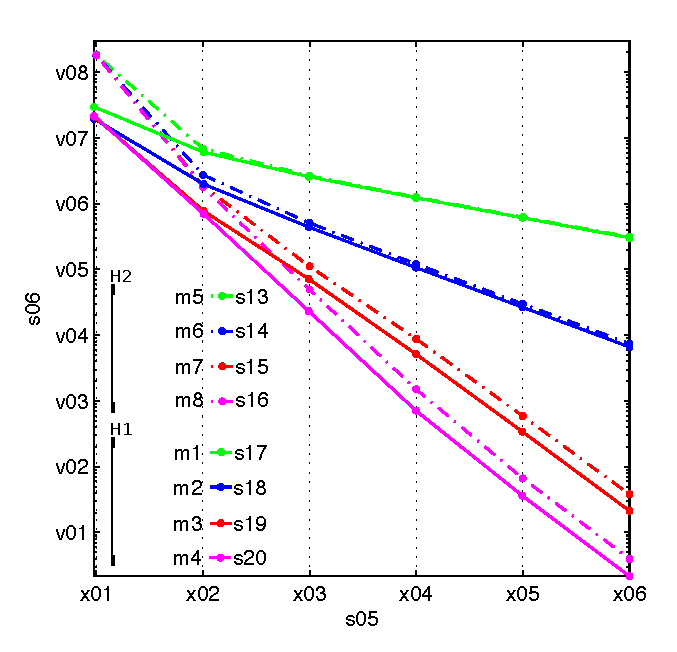
\includegraphics{L2comp.eps}}%
\end{psfrags}%
%
% End L2comp.tex
